\documentclass{article}

\usepackage{amsmath}
\usepackage{graphicx}
\usepackage{float}
\usepackage{fullpage}

% Default fixed font does not support bold face
\DeclareFixedFont{\ttb}{T1}{txtt}{bx}{n}{10} % for bold
\DeclareFixedFont{\ttm}{T1}{txtt}{m}{n}{10}  % for normal

% Custom colors
\usepackage{color}
\definecolor{deepblue}{rgb}{0,0,0.5}
\definecolor{deepred}{rgb}{0.6,0,0}
\definecolor{deepgreen}{rgb}{0,0.5,0}

\usepackage{listings}

% Python style for highlighting
\newcommand\pythonstyle{\lstset{
language=Python,
basicstyle=\ttm,
otherkeywords={self},             % Add keywords here
keywordstyle=\ttb\color{deepblue},
emph={MyClass,__init__},          % Custom highlighting
emphstyle=\ttb\color{deepred},    % Custom highlighting style
stringstyle=\color{deepgreen},
frame=tb,                         % Any extra options here
showstringspaces=false            % 
}}


% Python environment
\lstnewenvironment{python}[1][]
{
\pythonstyle
\lstset{#1}
}
{}

\title{Statistical Machine Learning: Assignment 1}
\author{Joris van Vugt, s4279859 \\ Luc Nies, s4136748}
\date{\today}

\begin{document}
\maketitle
\section{}

\subsection*{1.1}
\begin{python}
def f(x):
    return 1 + np.sin(6 * (x - 2))

def noisy_f(x):
    noise = np.random.normal(0, 0.3)
    return noise + f(x)

# Generate data
D = [noisy_f(x) for x in np.linspace(0, 1, 10)]
T = [noisy_f(x) for x in np.linspace(0, 1, 100)]
\end{python}
\begin{figure}[H]
\centering
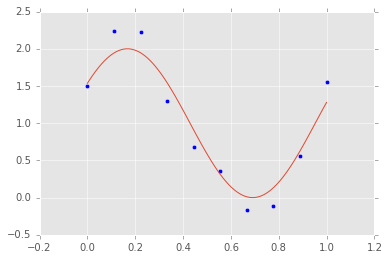
\includegraphics[width=.6\textwidth]{images/sin_d.png}
\caption{Plot of $f(x)$ and the 10 noisy observations in the training data}
\end{figure}

\pagebreak

\subsection*{1.2}
We can use \texttt{np.linalg.solve} to solve a set of linear equations in Python/NumPy. We use this function to solve
$$
\sum_{j=0}^M A_{ij}w_j = T_i
$$
with 
$$
A_{ij} = \sum_{n=1}^N x_n^{i + j} \hspace{1cm}
T_i = \sum_{n=1}^N t_n x_i^n
$$
Which gives the optimal weights for a dataset given the order of the polynomial M. Note that our code is for solving a polynomial of order $M - 1$.
\begin{python}
def pol_cur_fit(D, M):
    x = D[0, :]
    t = D[1, :]
    A = np.zeros((M, M))
    for i in range(M):
        for j in range(M):
            A[i, j] = np.sum(x ** (i+j))
    T = np.zeros(M)
    for i in range(M):
        T[i] = np.sum(t * x**i)
    w = np.linalg.solve(A, T)
    return w
\end{python}

\subsection*{1.3}
\begin{python}
def polynomial(X, w):
    return np.polyval(list(reversed(w)), X)

def RMSE(observed, target):
    error = 0.5 * np.sum((observed - target)**2)
    return np.sqrt(2*error / len(observed))
\end{python}
Note that \texttt{np.polyeval} expects the weights in reversed order from what we computed with \texttt{pol\_cur\_fit}.
\begin{figure}[H]
\centering
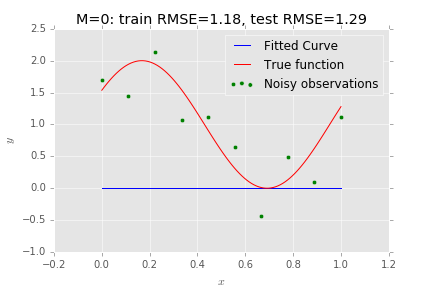
\includegraphics[width=.49\textwidth]{images/fit_m0_n_10.png}
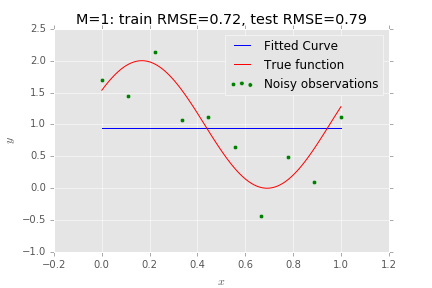
\includegraphics[width=.49\textwidth]{images/fit_m1_n_10.png}
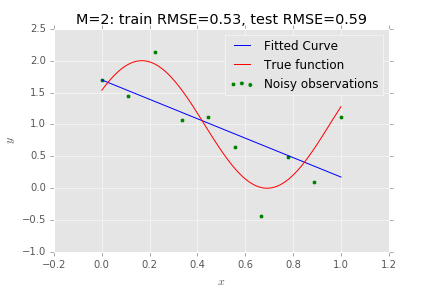
\includegraphics[width=.49\textwidth]{images/fit_m2_n_10.png}
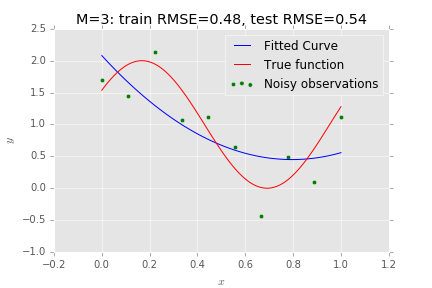
\includegraphics[width=.49\textwidth]{images/fit_m3_n_10.png}
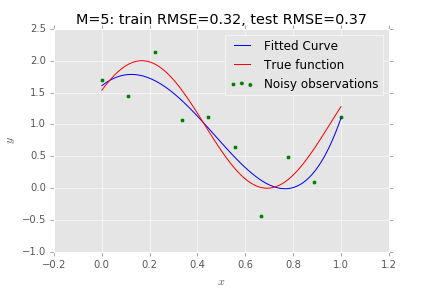
\includegraphics[width=.49\textwidth]{images/fit_m5_n_10.png}
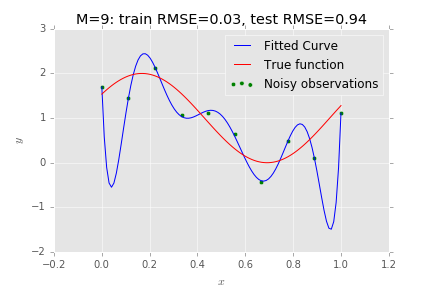
\includegraphics[width=.49\textwidth]{images/fit_m9_n_10.png}
\caption{Fitted curves for different values of M}
\end{figure}
When $M=2$, the polynomial is linear. From $M=4$ to $M=8$, the polynomial fits the underlying sine wave quite well. When $M=9$, the polynomial is clearly overfitted on the training data. This can also be concluded by comparing the root mean squared errors on the training and test sets.
\subsection*{1.4}
\begin{figure}[H]
\centering
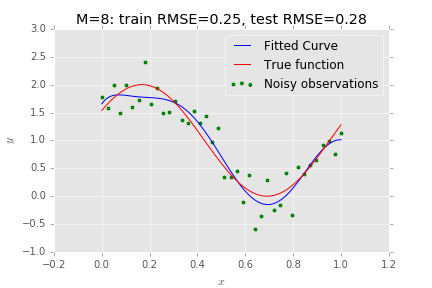
\includegraphics[width=0.6\textwidth]{images/fit_m8_n_40.png}
\caption{Fitted curve with $M=8$ and $N=40$}
\end{figure}
The fitted curves show less signs of overfitting overall and have lower errors. However for $M \geq 8$ there is still some overfitting to the noise, but since $N > M + 1$, the curve does not have enough degrees of freedom to fit all points exactly.
\subsection*{1.5}
\begin{table}[H]
\centering
\begin{tabular}{c | r | r}
$\textbf{w}$ & $\lambda=0$ & $\lambda=0.1$ \\
\hline
$w^*_0$ & 1.37 & 1.78 \\
$w^*_1$ & 61.59 & -1.19 \\
$w^*_2$ & -1022.49 & -1.29\\
$w^*_3$ & 7096.50 & -0.62 \\
$w^*_4$ & -25604.26 & -0.05 \\
$w^*_5$ & 51562.88 & 0.34 \\
$w^*_6$ & -58476.55 & 0.60 \\
$w^*_7$ & 34924.10 & 0.77 \\ 
$w^*_8$ & -8541.82 & 0.88 
\end{tabular}
\caption{Optimal weights for $M=9$ and $N=10$ with ($\lambda=0.1$)and without ($\lambda=0$) regularization}
\end{table}

The weigths with regularization are a lot smaller than the unregularized weights. There is also a smaller difference between the error on the test and the training set when using regularization.

\begin{figure}[H]
\centering
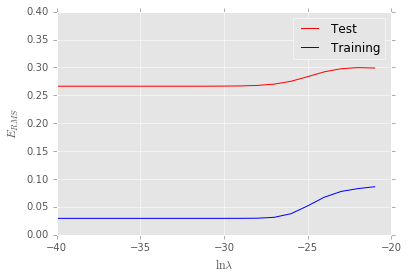
\includegraphics[width=0.6\textwidth]{images/effect_regularization.png}
\caption{The error on the training and test set versus the regularization strength}
\end{figure}
The reproduction of Figure 1.8 in Bishop looks slightly different for small values of $\ln \lambda$. We assume that the figure in Bishop is not on scale for $\ln \lambda < 35$ for educational purposes. We also noticed that this figure can vary a lot depending on the training and test set.

\section*{Exercise 2}
\subsection*{2.1}
\begin{figure}[H]
\centering
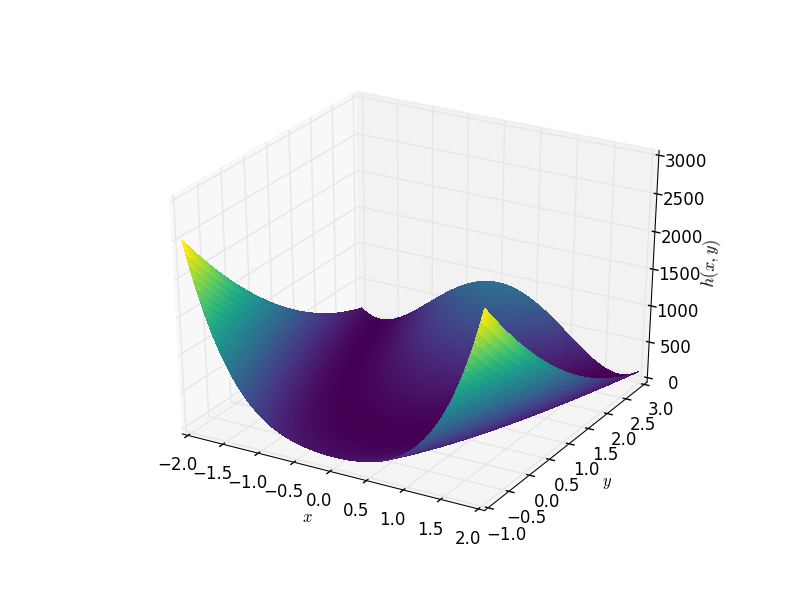
\includegraphics[width=.6\textwidth]{images/h.png}
\caption{Surface plot of $h(x, y)$}
\end{figure}
\begin{python}
def h(x, y):
    return 100 * (y - x**2)**2 + (1 - x)**2
\end{python}
We think that using gradient descent for this function will be slow, because there is a large `valley' (dark-blue area in the plot). The function also grows very rapidly outside the valley, which might make gradient descent more difficult because it will be difficult to find the right learning rate.
\subsection*{2.2}
We first calculate the gradient of the functions with respect to $x$ and $y$.
\begin{flalign}
h(x,y) &= 100(y-x^2)^2 + (1-x)^2 && \\
\frac{\partial h}{\partial y} &= 200(y-x^2) &&\\
\frac{\partial h}{\partial x} &= -400x(y-x^2) - 2 +2x \\
\end{flalign}

We now set $\frac{\partial h}{\partial y} = 0$ to find the minimum.
\begin{flalign}
200(y-x^2) &= 0 &&\\
200y &= 200x^2 &&\\
y &= x^2
\end{flalign}

Substitute the result in $\frac{\partial h}{\partial x}$ to find the $x$-coordinate of the minimum.
\begin{flalign}
-400x(y-x^2) - 2 + 2x &= 0 &&\\
-400x(x^2-x^2) - 2 + 2x &= 0 &&\\
-2 + 2x &= 0&&\\
2x &= 2&&\\
x &= 1
\end{flalign}

Lastly, we can use that to find the $y$-coordinate of the minimum.
\begin{flalign}
y &= 1^2 = 1 &&
\end{flalign}
So the minimum of $h$ is indeed at $(1, 1)$.
\subsection*{2.3}
We fill in the partial derivates of $h$ into $\textbf{x}_{n+1} = \textbf{x}_n - \eta \nabla E(\textbf{x}_n)$
\begin{flalign}
x_{n+1} &= x_n - \eta(-400x_n(y_n-x^2_n) - 2 + 2x_n)\\
y_{n+1} &= y_n - \eta(200(y_n-x^2_n))
\end{flalign}

\subsection*{2.4}
For small $\eta$ values ($\eta \leq 0.001$ in the tests we ran) gradient descent converges, but for larger values it quickly overshoots and never manages to converge. This is due to the rapid increase of $h$. It is hard to find a learning rate that scales well for the entire range of $h$. So when gradient descent overshoot, it will overcompensate and quickly diverge. The smaller the $\eta$ the more steps are needed.


\begin{figure}[H]
\centering
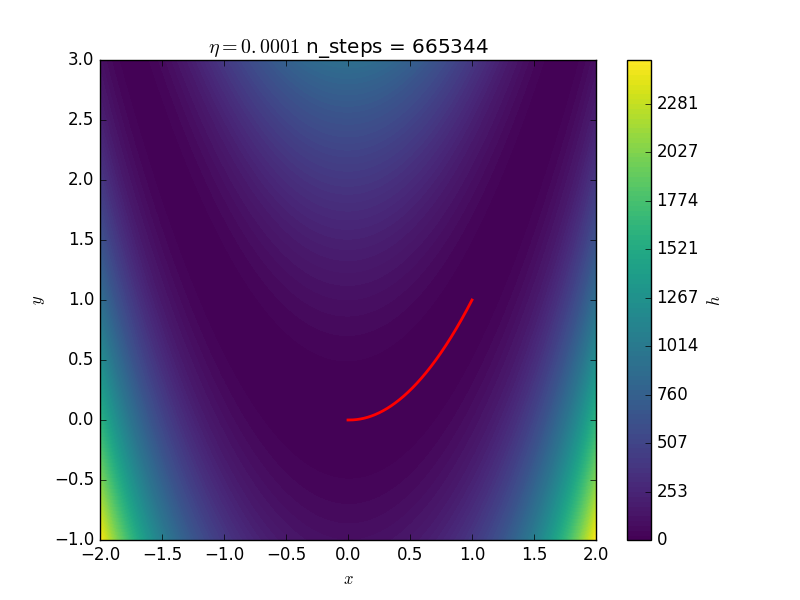
\includegraphics[width=.49\textwidth]{images/eta_0_0001.png}
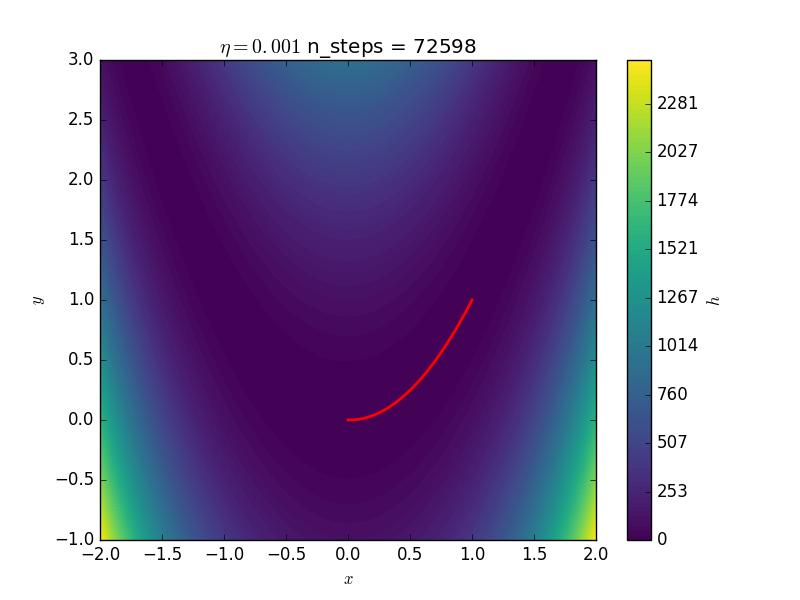
\includegraphics[width=.49\textwidth]{images/eta_0_001.png}
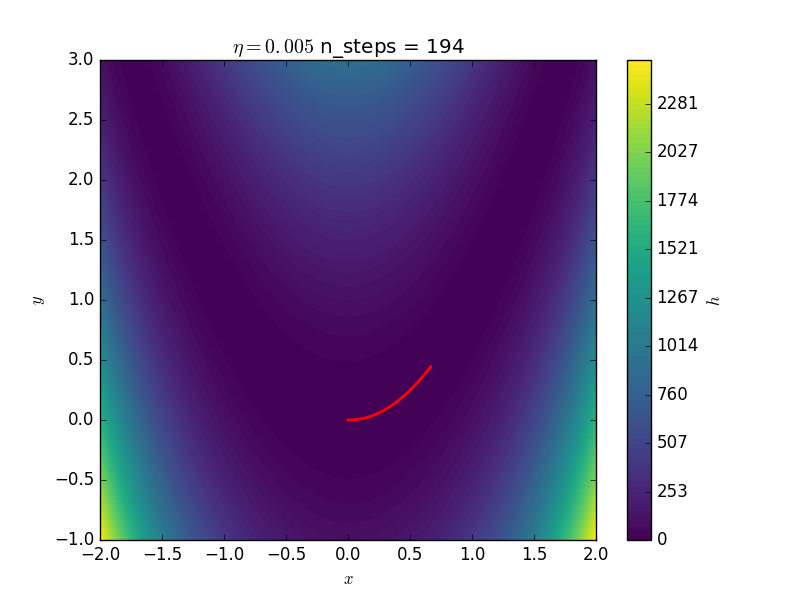
\includegraphics[width=.49\textwidth]{images/eta_0_005.png}
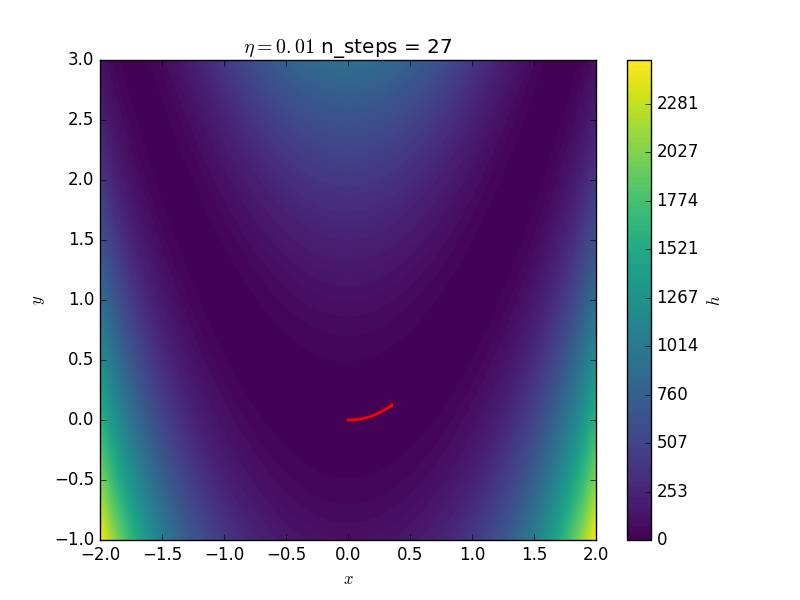
\includegraphics[width=.49\textwidth]{images/eta_0_01.png}
\caption{Gradient descent with different values or $\eta$, with start values $x = 0$ and $y = 0$}
\end{figure}

\begin{python}
def gradient_descent(eta = 0.005, start_x = 0, start_y = 0, max_iter = 500):
    x_list, y_list, h_list  = [start_x], [start_y], [h(start_x, start_y)]
    x = start_x
    y = start_y
    for _ in range(max_iter):
        x_temp = x - eta * (400 * x * (x**2-y) - 2 + 2 * x)
        y = y - eta * (200 * (y - x**2))
        x = x_temp
        h_new = h(x,y)
        if h_new >= h_list[-1]:
            break # Stop if h doesn't decrease anymore

        x_list.append(x)
        y_list.append(y)
        h_list.append(h(x,y))
        
    
    return x_list, y_list, h_list
\end{python}

\section*{3}
\subsection*{3.1}
\begin{flalign}
B &= \{1,2\} &&\\ 
F &=\{A,G\}
\end{flalign}
We want to calculate: $P(F_1=A | F_2=G)$. To this end, we first calculate the probability of picking a grapefruit from each box.
\begin{flalign}
P(F=A | B = 1) &= \frac{2}{3} &&\\
P(F=A | B = 2) &= \frac{5}{6} &&\\
P(F=G) &= P(F=G | B=1)P(B=1) + P(F=G | B=2)P(B=2) &&\\
&= \frac{1}{3} \times \frac{1}{2} + \frac{1}{6} \times \frac{1}{2} = \frac{1}{4} && \\
P(B =1 | F = G) &= \frac{P(F=G | B = 1)P(B=1)}{P(F = G)} &&\\
&= \frac{\frac{1}{3} \times \frac{1}{2}}{\frac{1}{4}} =\frac{2}{3}
\end{flalign}

\begin{flalign}
P(B=2 | F=G) &= 1 - P(B =1 | F = G) && \\
&= 1 - \frac{2}{3} = \frac{1}{3}
\end{flalign}

Intuitively, these are now the probabilities of each of the boxes.

\begin{flalign}
P(F_1 = A, | F_2 = G) &= P(F = A | B = 1)P(B=1|F=G) + P(F=A|B=2)P(B=2|F=G)\\
&= \frac{2}{3}\times \frac{2}{3} + \frac{1}{3} \times \frac{5}{6}\\
&= \frac{4}{9} + \frac{5}{18}\\
&= \frac{13}{18}
\end{flalign}
So the probablity that the first fruit is an apple given that the second fruit is a grapefruit is $\frac{13}{18}$.
It is less likely that a fruit picked from box 1 is an apple than when it was picked from box 2. If the second fruit is a grapefruit, it is more likely that it is picked from box 1, making it less likely that the first fruit is an apple.

\subsection*{3.2}
The new proboality of picking a grapefruit from box 1 is:
\begin{flalign}
P(F=G | B = 1 ) = \frac{4}{24} = \frac{1}{6}= P(F=G | B =2) && 
\end{flalign}
So from this, it follows that $P(B=1|F=G) = P(B=2|F=G) = \frac{1}{2}$. Since the probabilities of picking a grapefruit from both boxes are equal, it does not tell us anything about which box is now more likely.\\
The two picks are still dependent, as the other two fruits have different probablities per box. So if the first pick is an orange, it still tells us something about the second pick.

\end{document}